\documentclass[10pt]{report}

\usepackage{geometry}
\geometry{
	letterpaper,
	hmargin=0.7in,
	vmargin=1in,
	footskip=0.25in
}

\usepackage{enumerate} % for enumerate counter
\usepackage{subcaption} % for subfigures
\usepackage{amsthm} % for QED
\usepackage{mathtools} % for delimiter

\usepackage{listings} % for code
\lstset{ 
	language=R,
	basicstyle=\footnotesize\ttfamily,
	numbers=none,
	stepnumber=1,
	numbersep=8pt,
	showspaces=false,
	showstringspaces=false,
	showtabs=false,
	frame=single,
	tabsize=2,
	captionpos=t,
	breaklines=true,
	breakatwhitespace=false
} 

\usepackage{float} % for figure [H]
\usepackage{booktabs} % for tabular
\usepackage{caption} % for \caption*
\usepackage[export]{adjustbox} % for valign=t
\usepackage{array} % for column type m
\usepackage{verbatim}
\usepackage{graphicx}
%\graphicspath{ {imgs/} }

\usepackage{fancyhdr}
\pagestyle{fancy}
\fancyhead[L]{\hwAuther}
\fancyhead[C]{\courseNo}
\fancyhead[R]{\hwNo}

\usepackage{amssymb}
\usepackage{amsmath}

%Cover
\newcommand{\courseTitle}{Introduction to Mathematical Modeling}
\newcommand{\courseNo}{Math 380}
\newcommand{\hwAuther}{Zhihao Ai}

\newcommand{\hwNo}{HW \#9}
\newcommand{\hwDate}{Due on 04/10}

\title{
	\courseTitle\\
	\hwNo\\
	\hwDate
}
\author{\hwAuther}
\date{}
%

%Custom
%\everymath{\displaystyle}
\setlength\parindent{0pt}

%Custom commands
\newcommand{\ds}{\displaystyle}
\newcommand{\ts}{\textstyle}

\newcolumntype{N}{>$ c <$} 
\newcolumntype{M}[1]{>{\centering\arraybackslash $}m{#1}<{$}}

\newcommand{\abs}[1] {\left| #1 \right|}

\DeclarePairedDelimiter\autoparen{(}{)}
\newcommand{\pa}[1]{\autoparen*{#1}}

\newcommand{\var} {\text{var}}

\newcommand{\m}[1] {\mathbf{#1}}

\begin{document}

\maketitle

\begin{enumerate}
	\item 
	Define
	\[
	f(x) = 
	\begin{cases}
		1 & \text{three components of $x$ are greater than or equal to 0.5}\\
		0 & \text{otherwise}
	\end{cases}
	\]
	where $x$ is a vector consisting of five numbers from 0 to 1.\\
	Input: $n$ random $x$ to be generated\\
	Output: 
	Estimate of the probability $\hat{p}$ of three heads occuring when five fair coins are flipped
	\begin{enumerate}[i.]
		\item
		Initialize $c=0$
		
		\item
		For $i=1, \dots, n$, do steps 2a-b
		\begin{enumerate}[a.]
			\item 
			Generate five random numbers ranging from 0 to 1 constituting $x$
			
			\item 
			If $f(x) = 1$, then $c=c+1$
		\end{enumerate}
		
		\item
		$\hat{p} = c/n$
	\end{enumerate}
	Running the algorithm with $n$ being 1,000, 10,000 and 100,000, we have $\hat{p}$ being 0.307, 0.3095 and 0.31203, respectively.
	
	\item 
	Assuming Player 1 always calls "even", define
	\[
	f(x) = 
	\begin{cases}
	1 & \text{both components of $x$ are the same}\\
	-1 & \text{otherwise}
	\end{cases}
	\]
	where $x$ is a vector consisting of two numbers $\in \{0, 1\}$.\\
	Input: $n$ random $x$ to be generated\\
	Output: 
	Estimate of the money $m$ Player 1 has at the end of the game
	\begin{enumerate}[i.]
		\item
		Initialize $m=0$
		
		\item
		For $i=1, \dots, n$, do steps 2a-b
		\begin{enumerate}[a.]
			\item 
			Generate two random numbers $\in \{0, 1\}$ constituting $x$
			
			\item 
			$m = m + f(x)$
		\end{enumerate}
	\end{enumerate}
	Running the algorithm with $n$ being 1,000, 10,000 and 100,000, we have $m$ being -16, -116, and 292, respectively.
	
	\item 
	Since the largest value in the table is 281,416,000, we estimate $M$ to be 282,000,000. Using ordinary linear regression to fit the data, we have
	\begin{figure}[H]
		\centering
		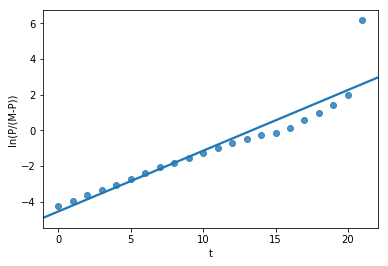
\includegraphics[width=0.5\linewidth]{3.png}
	\end{figure}
	The slope $rM$ is approximately 0.34. Since $M$ is 282,000,000, $r$ is $1.2\times 10^{-9}$. Then
	\[
	t^* = t_0 - \frac{1}{rM} \ln \frac{P_0}{M-P_0} = 0 - \frac{1}{0.34} \ln \frac{3929000}{282000000 - 3929000} = 12.53
	\]
	meaning 12.53 decades after 1790, which is about 1915. Using the model
	\[
	P(t) = \frac{M}{1+e^{-rM(t-t^*)}} = \frac{282000000}{1+e^{-0.34(t-12.53)}}
	\]
	the prediction in 1951 (6.1 decades after 1790) is calculated to be 158234518.
	
	\item 
	\begin{enumerate}
		\item 
		The first assumption is the spreading of the disease is limited by the maximum population $N$. It's reasonable because the island is isolated and there would be no people from elsewhere reach the island. Another assumption is that all people on the island are equally likely to be infected by the disease and the situation will remain unchanged. This assumption is not that valid but it is a reasonable assumption to simplify the problem, otherwise it would be too complicated.
		
		\item 
		Assuming $k=0.00005$ and $N=5000$, we have the graph of $dX/dt$ against $X$ as follows:
		\begin{figure}[H]
			\centering
			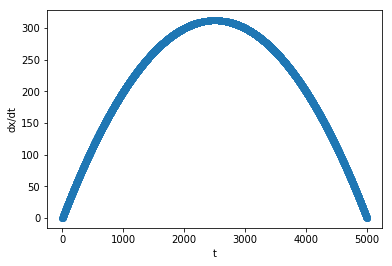
\includegraphics[width=0.5\linewidth]{4b.png}
		\end{figure}
	
		\item 
		For $x_1 = 1000 < N/2$, the graph would be
		\begin{figure}[H]
			\centering
			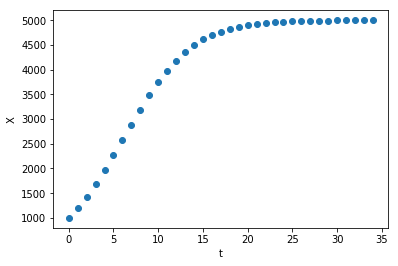
\includegraphics[width=0.5\linewidth]{4c1.png}
		\end{figure}
		For $x_2 = 4000 > N/2$, the graph would be
		\begin{figure}[H]
			\centering
			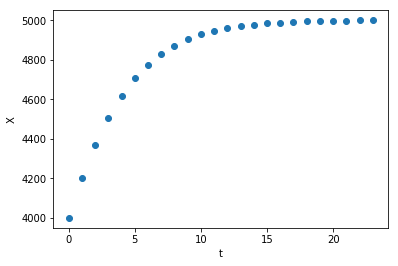
\includegraphics[width=0.5\linewidth]{4c2.png}
		\end{figure}
	
		\item 
		According to equation (10-11), the function is
		\[
		X(t) = \frac{N X_0 e^{kN(t-t_0)}}{N - X_0 + X_0 e^{-kN(t-t_0)}}
		\]
		
		\item 
		Rewrite the function in part (d) and we have
		\[
		X(t) = \frac{N X_0}{X_0 + (N - X_0) e^{-kN(t-t_0)}}
		\]
		As $t \to \infty$, $e^{-kN(t-t_0)} \to 0$ and $X(t) \to M$.
		
		\item 
		Because $\ln (X/(N-X)) = kNt + C$, we have
		\begin{align*}
			2kN + C &= -0.5\\
			6kN + C &= 1.5\\
			10kN + C &= 3.5
		\end{align*}
		Solving it, we have $k=0.0001$ and $C = -1.5$. So the collected data support the given model.
		
		\item 
		Since $k=0.0001$ and $C = -1.5$, 
		\[
		t^* = - \frac{C}{kN} = 3
		\]
		According to formula (10-12), the number of people infected by $t=12$ days would be
		\[
		X(12) = \frac{N}{1 + e^{-k N (t-t^*)}} = \frac{5000}{1 + e^{-0.0001 \cdot 5000 (12-3)}} \approx 4945
		\]
		
	\end{enumerate}
\end{enumerate}

\end{document}

